\documentclass{article}\usepackage[]{graphicx}\usepackage[]{color}
% maxwidth is the original width if it is less than linewidth
% otherwise use linewidth (to make sure the graphics do not exceed the margin)
\makeatletter
\def\maxwidth{ %
  \ifdim\Gin@nat@width>\linewidth
    \linewidth
  \else
    \Gin@nat@width
  \fi
}
\makeatother

\definecolor{fgcolor}{rgb}{0.345, 0.345, 0.345}
\newcommand{\hlnum}[1]{\textcolor[rgb]{0.686,0.059,0.569}{#1}}%
\newcommand{\hlstr}[1]{\textcolor[rgb]{0.192,0.494,0.8}{#1}}%
\newcommand{\hlcom}[1]{\textcolor[rgb]{0.678,0.584,0.686}{\textit{#1}}}%
\newcommand{\hlopt}[1]{\textcolor[rgb]{0,0,0}{#1}}%
\newcommand{\hlstd}[1]{\textcolor[rgb]{0.345,0.345,0.345}{#1}}%
\newcommand{\hlkwa}[1]{\textcolor[rgb]{0.161,0.373,0.58}{\textbf{#1}}}%
\newcommand{\hlkwb}[1]{\textcolor[rgb]{0.69,0.353,0.396}{#1}}%
\newcommand{\hlkwc}[1]{\textcolor[rgb]{0.333,0.667,0.333}{#1}}%
\newcommand{\hlkwd}[1]{\textcolor[rgb]{0.737,0.353,0.396}{\textbf{#1}}}%
\let\hlipl\hlkwb

\usepackage{framed}
\makeatletter
\newenvironment{kframe}{%
 \def\at@end@of@kframe{}%
 \ifinner\ifhmode%
  \def\at@end@of@kframe{\end{minipage}}%
  \begin{minipage}{\columnwidth}%
 \fi\fi%
 \def\FrameCommand##1{\hskip\@totalleftmargin \hskip-\fboxsep
 \colorbox{shadecolor}{##1}\hskip-\fboxsep
     % There is no \\@totalrightmargin, so:
     \hskip-\linewidth \hskip-\@totalleftmargin \hskip\columnwidth}%
 \MakeFramed {\advance\hsize-\width
   \@totalleftmargin\z@ \linewidth\hsize
   \@setminipage}}%
 {\par\unskip\endMakeFramed%
 \at@end@of@kframe}
\makeatother

\definecolor{shadecolor}{rgb}{.97, .97, .97}
\definecolor{messagecolor}{rgb}{0, 0, 0}
\definecolor{warningcolor}{rgb}{1, 0, 1}
\definecolor{errorcolor}{rgb}{1, 0, 0}
\newenvironment{knitrout}{}{} % an empty environment to be redefined in TeX

\usepackage{alltt}
\usepackage{Sweave}
\usepackage{float}
\usepackage{subcaption}
\usepackage{graphicx}
\usepackage{tabularx}
\usepackage{siunitx}
\usepackage{multirow}
\usepackage{amssymb} % for math symbols
\usepackage{amsmath} % for aligning equations
%\usepackage{hyperref}
\usepackage{textcomp}
\usepackage{mdframed}
\usepackage{longtable}
\usepackage{natbib}
\bibliographystyle{..//references/styles/besjournalsnew.bst}
%\usepackage[hyphens]{url}
\usepackage{caption}
\setlength{\captionmargin}{30pt}
\setlength{\abovecaptionskip}{0pt}
\setlength{\belowcaptionskip}{10pt}
\topmargin -1.5cm        
\oddsidemargin -0.04cm   
\evensidemargin -0.04cm
\textwidth 16.59cm
\textheight 21.94cm 
%\pagestyle{empty} %comment if want page numbers
\parskip 7.2pt
\renewcommand{\baselinestretch}{1}
\parindent 0pt
\usepackage{lineno}
\linenumbers

%cross referencing:
\usepackage{xr}
\externaldocument{chillfrz_outline}

\newmdenv[
  topline=true,
  bottomline=true,
  skipabove=\topsep,
  skipbelow=\topsep
]{siderules}

%% R Script


\IfFileExists{upquote.sty}{\usepackage{upquote}}{}
\begin{document}

\noindent \textbf{\Large{Supplemental materials: False spring damage on temperate tree seedlings is amplified with winter warming}}

\noindent Authors:\\
C. J. Chamberlain $^{1,2}$, K. Woodruff $^{1}$ \& E. M. Wolkovich $^{1,2,3}$
\vspace{2ex}\\
\emph{Author affiliations:}\\
$^{1}$Arnold Arboretum of Harvard University, 1300 Centre Street, Boston, Massachusetts, USA 02131; \\
$^{2}$Organismic \& Evolutionary Biology, Harvard University, 26 Oxford Street, Cambridge, Massachusetts, USA 02138; \\
$^{3}$Forest \& Conservation Sciences, Faculty of Forestry, University of British Columbia, 2424 Main Mall, Vancouver, BC V6T 1Z4\\
\vspace{2ex}
$^*$Corresponding author: 248.953.0189; cchamberlain@g.harvard.edu\\

\renewcommand{\thetable}{S\arabic{table}}
\renewcommand{\thefigure}{S\arabic{figure}}
\renewcommand{\labelitemi}{$-$}
\setkeys{Gin}{width=0.8\textwidth}



\section*{Supplemental Materials and Methods: Data analysis and model equations}
Using Bayesian hierarchicial models, we estimated the effects of chilling duration, false spring treatment and all two-way interactions as predictors with species modeled hierarchically as grouping factors. False spring treatment is written as `tx' in the equation below and chilling was split into two binary predictors: `chill1', which is denoted as `0' for 4 weeks of chilling or `1' for 6 weeks of chilling and `chill2' which is `1' for 8 weeks of chilling:

\begin{align*}
y_i &= \alpha_{species[i]} + \beta_{tx_{species[i]}}X_{tx} + \beta_{chill1_{species[i]}}X_{chill1} + \beta_{chill2_{species[i]}}X_{chill2}\\
&+ \beta_{txchill1_{species[i]}}X_{txchill1} + \beta_{txchill2_{species[i]}}X_{txchill2} + \epsilon_i \tag{1}\\,
\end{align*}
\begin{align*}
\epsilon_i & \sim N(0,\sigma_y) \\
\end{align*}

The $\alpha$ and each of the five $\beta$ coefficients are modeled at the species level, as follows:

\begin{align*}
\alpha_{species} & \sim N(\mu_{\alpha}, \sigma_{\alpha}) \\
\beta_{tx_{species}} & \sim N(\mu_{tx}, \sigma_{tx}) \\
\beta_{chill1_{species}} & \sim N(\mu_{chill1}, \sigma_{chill1}) \\
\beta_{chill2_{species}} & \sim N(\mu_{chill2}, \sigma_{chill2}) \\
\beta_{txchill1_{species}} & \sim N(\mu_{txchill1}, \sigma_{txchill1}) \\
\beta_{txchill2_{species}} & \sim N(\mu_{txchill2}, \sigma_{txchill2}) \\
\end{align*}

where $i$ represents each unique observation, $species$ is the species, $\alpha$ represents the intercept, $\beta$ terms represent slope estimates, and $y$ is the phenology or growth measurement. 

For the shoot apical meristem model, we used a Bernouilli distribution, which is modeled as:

\begin{align*}
 y_i & \sim Binomial(1,p) \tag{2} \\
logit(p) &= \alpha_{species[i]} + \beta_{tx_{species[i]}}X_{tx} + \beta_{chill1_{species[i]}}X_{chill1} + \beta_{chill2_{species[i]}}X_{chill2}\\
&+ \beta_{txchill1_{species[i]}}X_{txchill1} + \beta_{txchill2_{species[i]}}X_{txchill2} + \epsilon_i \nonumber\\,
\end{align*}

The $\alpha$ and each of the five $\beta$ coefficients are modeled the same as the other models:

\begin{align*}
\alpha_{species} & \sim N(\mu_{\alpha}, \sigma_{\alpha}) \\
\beta_{tx_{species}} & \sim N(\mu_{tx}, \sigma_{tx}) \\
\beta_{chill1_{species}} & \sim N(\mu_{chill1}, \sigma_{chill1}) \\
\beta_{chill2_{species}} & \sim N(\mu_{chill2}, \sigma_{chill2}) \\
\beta_{txchill1_{species}} & \sim N(\mu_{txchill1}, \sigma_{txchill1}) \\
\beta_{txchill2_{species}} & \sim N(\mu_{txchill2}, \sigma_{txchill2}) \\
\end{align*}

Model estimates for the shoot apical meristem model were modeled on the logit scale (shown in all tables) and were converted to probability percentages in all figures for easier interpretation by following the `divide by four' rule \citep{Gelman2006}.

\bibliography{..//references/chillfreeze.bib}

\section*{Supplemental tables and figures}

% latex table generated in R 3.6.0 by xtable 1.8-4 package
% Tue Aug 18 10:33:34 2020
\begin{table}[H]
\centering
\caption{Summary of simple linear regression model of day of budburst across chilling treatments.} 
\label{tab:simpbb}
\begin{tabular}{lrr}
  \hline
term & mean & std.err \\ 
  \hline
Intercept & 28.58 & 1.22 \\ 
  Chilling 6 Wks & -2.79 & 1.74 \\ 
  Chilling 8 Wks & -7.63 & 1.76 \\ 
   \hline
\end{tabular}
\end{table}
% latex table generated in R 3.6.0 by xtable 1.8-4 package
% Tue Aug 18 10:33:34 2020
\begin{table}[H]
\centering
\caption{Summary of simple linear regression model of duration of vegetative across chilling treatments.} 
\label{tab:simpdvr}
\begin{tabular}{lrr}
  \hline
term & mean & std.err \\ 
  \hline
Intercept & 18.35 & 0.54 \\ 
  Chilling 6 Wks & -2.07 & 0.77 \\ 
  Chilling 8 Wks & -2.72 & 0.78 \\ 
   \hline
\end{tabular}
\end{table}


\newpage
% latex table generated in R 3.6.0 by xtable 1.8-4 package
% Tue Aug 18 10:33:34 2020
\begin{longtable}{lrrrrrrr}
\caption{Summary of model with the effects of false spring treatment and chilling duration across species on duration of vegetative risk.} \\ 
  \hline
 & mean & 2\% & 10\% & 25\% & 75\% & 90\% & 98\% \\ 
  \hline \endhead  \hline
Intercept & 16.02 & 12.46 & 13.60 & 15.08 & 16.90 & 18.52 & 20.23 \\ 
  Tx & 2.97 & 1.13 & 1.68 & 2.45 & 3.49 & 4.26 & 4.87 \\ 
  Chill 6 Wks & -0.53 & -3.83 & -2.73 & -1.38 & 0.32 & 1.72 & 2.99 \\ 
  Chill 8 Wks & -2.67 & -5.54 & -4.56 & -3.35 & -1.94 & -0.85 & 0.03 \\ 
  Tx:Chill 6 Wks & -0.91 & -3.59 & -2.78 & -1.65 & -0.17 & 0.92 & 1.85 \\ 
  Tx:Chill 8 Wks & 0.62 & -1.97 & -1.14 & -0.08 & 1.34 & 2.38 & 3.25 \\ 
  \textit{Acer saccharinum},Intercept & -3.06 & -7.74 & -5.82 & -4.12 & -1.93 & -0.40 & 0.75 \\ 
  \textit{Alnus incana rugosa},Intercept & 4.39 & 0.17 & 1.66 & 3.33 & 5.44 & 7.19 & 8.51 \\ 
  \textit{Betula papyrifera},Intercept & 0.96 & -3.52 & -1.86 & -0.06 & 2.02 & 3.69 & 4.85 \\ 
  \textit{Betula populifolia},Intercept & 0.20 & -4.12 & -2.47 & -0.86 & 1.27 & 2.93 & 4.19 \\ 
  \textit{Cornus racemosa},Intercept & 0.48 & -3.87 & -2.35 & -0.54 & 1.57 & 3.10 & 4.26 \\ 
  \textit{Salix purpurea},Intercept & -5.49 & -10.38 & -8.46 & -6.57 & -4.33 & -2.69 & -1.40 \\ 
  \textit{Sorbus americana},Intercept & -1.14 & -5.56 & -3.88 & -2.20 & -0.07 & 1.60 & 2.79 \\ 
  \textit{Viburnum dendatum},Intercept & 3.57 & -0.78 & 0.80 & 2.51 & 4.67 & 6.29 & 7.69 \\ 
  \textit{Acer saccharinum},Tx & -0.36 & -2.80 & -1.82 & -0.72 & 0.05 & 0.63 & 1.27 \\ 
  \textit{Alnus incana rugosa},Tx & 0.37 & -1.36 & -0.73 & -0.06 & 0.76 & 1.91 & 2.86 \\ 
  \textit{Betula papyrifera},Tx & 0.45 & -1.17 & -0.54 & -0.03 & 0.84 & 2.03 & 3.08 \\ 
  \textit{Betula populifolia},Tx & -0.43 & -3.09 & -1.97 & -0.80 & 0.04 & 0.55 & 1.12 \\ 
  \textit{Cornus racemosa},Tx & 0.00 & -1.93 & -1.15 & -0.29 & 0.32 & 1.13 & 1.91 \\ 
  \textit{Salix purpurea},Tx & -0.14 & -2.48 & -1.59 & -0.55 & 0.25 & 1.21 & 2.14 \\ 
  \textit{Sorbus americana},Tx & -0.21 & -2.43 & -1.57 & -0.54 & 0.15 & 0.84 & 1.57 \\ 
  \textit{Viburnum dendatum},Tx & 0.35 & -1.38 & -0.75 & -0.10 & 0.74 & 1.93 & 2.86 \\ 
  \textit{Acer saccharinum},Chill 6 Wks & -0.13 & -4.23 & -2.82 & -1.21 & 0.92 & 2.61 & 4.04 \\ 
  \textit{Alnus incana rugosa},Chill 6 Wks & -0.66 & -4.71 & -3.50 & -1.71 & 0.41 & 2.10 & 3.53 \\ 
  \textit{Betula papyrifera},Chill 6 Wks & 1.50 & -2.35 & -1.14 & 0.40 & 2.54 & 4.30 & 5.65 \\ 
  \textit{Betula populifolia},Chill 6 Wks & -0.59 & -4.77 & -3.43 & -1.62 & 0.50 & 2.10 & 3.22 \\ 
  \textit{Cornus racemosa},Chill 6 Wks & 0.46 & -3.46 & -2.14 & -0.56 & 1.48 & 3.11 & 4.43 \\ 
  \textit{Salix purpurea},Chill 6 Wks & 4.60 & 0.55 & 1.62 & 3.26 & 5.84 & 7.88 & 9.27 \\ 
  \textit{Sorbus americana},Chill 6 Wks & -2.20 & -6.59 & -5.11 & -3.27 & -1.02 & 0.45 & 1.44 \\ 
  \textit{Viburnum dendatum},Chill 6 Wks & -3.19 & -7.67 & -6.24 & -4.28 & -2.01 & -0.48 & 0.62 \\ 
  \textit{Acer saccharinum},Chill 8 Wks & 0.94 & -2.40 & -1.30 & -0.02 & 1.85 & 3.42 & 4.57 \\ 
  \textit{Alnus incana rugosa},Chill 8 Wks & -1.32 & -5.07 & -3.77 & -2.23 & -0.38 & 1.04 & 2.09 \\ 
  \textit{Betula papyrifera},Chill 8 Wks & 0.21 & -3.49 & -2.22 & -0.68 & 1.12 & 2.52 & 3.77 \\ 
  \textit{Betula populifolia},Chill 8 Wks & -1.36 & -5.28 & -3.90 & -2.25 & -0.39 & 0.82 & 1.82 \\ 
  \textit{Cornus racemosa},Chill 8 Wks & 0.61 & -2.76 & -1.58 & -0.30 & 1.48 & 2.94 & 4.23 \\ 
  \textit{Salix purpurea},Chill 8 Wks & 3.91 & 0.30 & 1.23 & 2.72 & 5.00 & 6.79 & 8.30 \\ 
  \textit{Sorbus americana},Chill 8 Wks & -0.51 & -4.16 & -2.86 & -1.41 & 0.41 & 1.76 & 2.89 \\ 
  \textit{Viburnum dendatum},Chill 8 Wks & -2.54 & -6.43 & -5.09 & -3.50 & -1.50 & -0.18 & 0.69 \\ 
  \textit{Acer saccharinum},Tx:Chill 6 Wks & -0.46 & -4.34 & -2.80 & -0.98 & 0.16 & 1.15 & 2.08 \\ 
  \textit{Alnus incana rugosa},Tx:Chill 6 Wks & 0.35 & -2.54 & -1.42 & -0.27 & 0.89 & 2.66 & 4.38 \\ 
  \textit{Betula papyrifera},Tx:Chill 6 Wks & 0.33 & -2.71 & -1.36 & -0.22 & 0.85 & 2.44 & 3.77 \\ 
  \textit{Betula populifolia},Tx:Chill 6 Wks & -0.54 & -4.45 & -2.83 & -1.05 & 0.11 & 1.06 & 2.03 \\ 
  \textit{Cornus racemosa},Tx:Chill 6 Wks & 0.23 & -2.65 & -1.45 & -0.26 & 0.69 & 2.25 & 3.58 \\ 
  \textit{Salix purpurea},Tx:Chill 6 Wks & 1.07 & -1.87 & -0.80 & 0.02 & 1.84 & 4.03 & 5.96 \\ 
  \textit{Sorbus americana},Tx:Chill 6 Wks & -0.44 & -3.99 & -2.60 & -0.97 & 0.16 & 1.13 & 2.24 \\ 
  \textit{Viburnum dendatum},Tx:Chill 6 Wks & -0.58 & -4.61 & -2.97 & -1.16 & 0.10 & 1.07 & 2.17 \\ 
  \textit{Acer saccharinum},Tx:Chill 8 Wks & -0.05 & -2.85 & -1.67 & -0.45 & 0.33 & 1.47 & 2.79 \\ 
  \textit{Alnus incana rugosa},Tx:Chill 8 Wks & 0.12 & -2.75 & -1.46 & -0.30 & 0.54 & 1.87 & 3.40 \\ 
  \textit{Betula papyrifera},Tx:Chill 8 Wks & 0.31 & -1.95 & -1.01 & -0.16 & 0.72 & 2.14 & 3.56 \\ 
  \textit{Betula populifolia},Tx:Chill 8 Wks & -0.06 & -2.98 & -1.62 & -0.43 & 0.33 & 1.43 & 2.66 \\ 
  \textit{Cornus racemosa},Tx:Chill 8 Wks & 0.40 & -1.62 & -0.83 & -0.10 & 0.75 & 2.28 & 3.86 \\ 
  \textit{Salix purpurea},Tx:Chill 8 Wks & -0.09 & -3.49 & -2.09 & -0.58 & 0.43 & 1.75 & 2.95 \\ 
  \textit{Sorbus americana},Tx:Chill 8 Wks & -0.48 & -4.01 & -2.61 & -0.90 & 0.08 & 0.80 & 1.61 \\ 
  \textit{Viburnum dendatum},Tx:Chill 8 Wks & -0.25 & -3.57 & -2.24 & -0.67 & 0.26 & 1.25 & 2.36 \\ 
   \hline
\hline
\label{tab:suppmoddvr}
\end{longtable}


\newpage
% latex table generated in R 3.6.0 by xtable 1.8-4 package
% Tue Aug 18 10:33:34 2020
\begin{longtable}{lrrrrrrr}
\caption{Summary of model with the effects of false spring treatment and chilling duration across species on growing season length.} \\ 
  \hline
 & mean & 2\% & 10\% & 25\% & 75\% & 90\% & 98\% \\ 
  \hline \endhead  \hline
Intercept & 283.95 & 249.62 & 263.13 & 276.95 & 291.73 & 302.64 & 310.98 \\ 
  Tx & -0.32 & -14.91 & -9.61 & -3.88 & 3.30 & 8.70 & 13.24 \\ 
  Chill 6 Wks & 2.48 & -8.70 & -5.40 & -0.78 & 5.64 & 10.60 & 14.02 \\ 
  Chill 8 Wks & -9.66 & -21.36 & -17.91 & -12.97 & -6.36 & -1.56 & 2.78 \\ 
  Tx:Chill 6 Wks & -14.87 & -30.38 & -25.87 & -19.39 & -10.39 & -4.08 & 0.58 \\ 
  Tx:Chill 8 Wks & -8.57 & -26.11 & -20.52 & -13.22 & -3.93 & 2.97 & 8.55 \\ 
  \textit{Acer saccharinum},Intercept & -10.08 & -38.20 & -29.41 & -18.27 & -2.60 & 11.77 & 24.62 \\ 
  \textit{Alnus incana rugosa},Intercept & 34.87 & 6.79 & 15.33 & 26.40 & 42.61 & 56.76 & 71.28 \\ 
  \textit{Betula papyrifera},Intercept & 8.84 & -18.52 & -10.75 & 0.69 & 16.27 & 30.38 & 43.52 \\ 
  \textit{Betula populifolia},Intercept & 33.10 & 6.24 & 13.92 & 24.78 & 40.58 & 54.73 & 67.96 \\ 
  \textit{Cornus racemosa},Intercept & -22.76 & -50.18 & -42.58 & -30.94 & -15.15 & -1.52 & 10.97 \\ 
  \textit{Salix purpurea},Intercept & 38.58 & 10.89 & 19.10 & 30.08 & 45.87 & 60.65 & 73.96 \\ 
  \textit{Sorbus americana},Intercept & -38.34 & -66.08 & -58.11 & -46.41 & -30.66 & -17.21 & -5.41 \\ 
  \textit{Viburnum dendatum},Intercept & 10.47 & -17.45 & -8.43 & 2.20 & 17.88 & 32.32 & 45.39 \\ 
  \textit{Acer saccharinum},Tx & 0.48 & -13.31 & -8.48 & -2.65 & 3.50 & 9.98 & 15.99 \\ 
  \textit{Alnus incana rugosa},Tx & 3.43 & -10.16 & -5.56 & -0.26 & 6.82 & 14.28 & 20.26 \\ 
  \textit{Betula papyrifera},Tx & 2.81 & -10.46 & -5.48 & -0.60 & 5.92 & 13.47 & 19.93 \\ 
  \textit{Betula populifolia},Tx & 3.94 & -9.87 & -4.75 & -0.05 & 7.44 & 15.08 & 20.93 \\ 
  \textit{Cornus racemosa},Tx & -4.95 & -22.59 & -16.02 & -8.55 & -0.62 & 3.61 & 8.59 \\ 
  \textit{Salix purpurea},Tx & 5.07 & -8.45 & -3.61 & 0.57 & 8.73 & 16.44 & 22.97 \\ 
  \textit{Sorbus americana},Tx & -9.46 & -30.44 & -22.95 & -14.30 & -3.43 & 0.68 & 3.58 \\ 
  \textit{Viburnum dendatum},Tx & 4.80 & -7.73 & -3.57 & 0.42 & 8.43 & 16.24 & 22.77 \\ 
  \textit{Acer saccharinum},Chill 6 Wks & 1.16 & -8.90 & -5.20 & -0.93 & 2.94 & 9.46 & 14.87 \\ 
  \textit{Alnus incana rugosa},Chill 6 Wks & -3.09 & -20.08 & -13.31 & -5.34 & 0.10 & 2.94 & 6.95 \\ 
  \textit{Betula papyrifera},Chill 6 Wks & 0.24 & -10.97 & -6.27 & -1.58 & 1.99 & 7.16 & 12.24 \\ 
  \textit{Betula populifolia},Chill 6 Wks & -0.95 & -15.17 & -8.97 & -2.88 & 1.09 & 5.84 & 10.95 \\ 
  \textit{Cornus racemosa},Chill 6 Wks & 2.10 & -7.28 & -3.91 & -0.36 & 4.11 & 11.14 & 17.59 \\ 
  \textit{Salix purpurea},Chill 6 Wks & -2.49 & -18.32 & -12.13 & -4.73 & 0.26 & 3.66 & 8.14 \\ 
  \textit{Sorbus americana},Chill 6 Wks & 2.48 & -8.47 & -4.22 & -0.38 & 4.85 & 12.27 & 18.17 \\ 
  \textit{Viburnum dendatum},Chill 6 Wks & -0.86 & -14.00 & -8.25 & -2.71 & 1.06 & 5.52 & 10.41 \\ 
  \textit{Acer saccharinum},Chill 8 Wks & 2.26 & -7.25 & -3.68 & -0.34 & 4.17 & 12.18 & 18.81 \\ 
  \textit{Alnus incana rugosa},Chill 8 Wks & -1.09 & -16.13 & -9.56 & -3.06 & 1.06 & 5.89 & 11.52 \\ 
  \textit{Betula papyrifera},Chill 8 Wks & -0.91 & -14.89 & -8.74 & -2.59 & 1.12 & 5.12 & 10.29 \\ 
  \textit{Betula populifolia},Chill 8 Wks & -0.95 & -15.15 & -9.10 & -2.78 & 1.07 & 5.71 & 10.63 \\ 
  \textit{Cornus racemosa},Chill 8 Wks & -0.85 & -15.44 & -9.03 & -2.70 & 1.25 & 5.75 & 10.64 \\ 
  \textit{Salix purpurea},Chill 8 Wks & -2.05 & -18.54 & -11.57 & -4.14 & 0.54 & 4.45 & 9.19 \\ 
  \textit{Sorbus americana},Chill 8 Wks & 1.65 & -10.95 & -5.72 & -0.87 & 3.86 & 11.56 & 18.34 \\ 
  \textit{Viburnum dendatum},Chill 8 Wks & 1.14 & -10.13 & -5.30 & -0.98 & 2.88 & 9.66 & 15.57 \\ 
  \textit{Acer saccharinum},Tx:Chill 6 Wks & -1.83 & -20.16 & -11.95 & -3.63 & 0.73 & 5.03 & 9.99 \\ 
  \textit{Alnus incana rugosa},Tx:Chill 6 Wks & 0.00 & -15.03 & -8.42 & -2.10 & 2.09 & 8.55 & 15.36 \\ 
  \textit{Betula papyrifera},Tx:Chill 6 Wks & -0.27 & -14.41 & -8.15 & -2.15 & 1.62 & 7.46 & 13.60 \\ 
  \textit{Betula populifolia},Tx:Chill 6 Wks & 0.93 & -12.03 & -6.77 & -1.41 & 2.96 & 10.16 & 17.80 \\ 
  \textit{Cornus racemosa},Tx:Chill 6 Wks & 0.11 & -14.72 & -8.28 & -2.04 & 2.17 & 8.70 & 15.64 \\ 
  \textit{Salix purpurea},Tx:Chill 6 Wks & -0.04 & -15.83 & -8.51 & -2.13 & 2.11 & 8.46 & 15.94 \\ 
  \textit{Sorbus americana},Tx:Chill 6 Wks & 0.64 & -15.11 & -7.97 & -2.03 & 3.01 & 10.74 & 17.88 \\ 
  \textit{Viburnum dendatum},Tx:Chill 6 Wks & 0.83 & -12.37 & -6.44 & -1.32 & 2.63 & 10.09 & 17.67 \\ 
  \textit{Acer saccharinum},Tx:Chill 8 Wks & 2.41 & -12.37 & -6.29 & -0.88 & 5.15 & 14.84 & 22.85 \\ 
  \textit{Alnus incana rugosa},Tx:Chill 8 Wks & 1.07 & -16.64 & -9.14 & -1.88 & 3.93 & 12.31 & 20.49 \\ 
  \textit{Betula papyrifera},Tx:Chill 8 Wks & 2.65 & -11.25 & -5.91 & -0.76 & 5.52 & 15.06 & 22.65 \\ 
  \textit{Betula populifolia},Tx:Chill 8 Wks & 0.32 & -16.97 & -10.49 & -2.47 & 3.00 & 11.13 & 18.57 \\ 
  \textit{Cornus racemosa},Tx:Chill 8 Wks & -0.64 & -18.64 & -11.44 & -3.57 & 2.09 & 9.71 & 17.07 \\ 
  \textit{Salix purpurea},Tx:Chill 8 Wks & 0.80 & -17.89 & -9.83 & -2.16 & 3.62 & 12.46 & 21.20 \\ 
  \textit{Sorbus americana},Tx:Chill 8 Wks & -6.00 & -33.31 & -23.19 & -10.33 & -0.07 & 3.65 & 8.57 \\ 
  \textit{Viburnum dendatum},Tx:Chill 8 Wks & 2.04 & -14.08 & -7.10 & -1.10 & 4.83 & 14.10 & 22.46 \\ 
   \hline
\hline
\label{tab:suppmodgs}
\end{longtable}


\newpage
% latex table generated in R 3.6.0 by xtable 1.8-4 package
% Tue Aug 18 10:33:34 2020
\begin{longtable}{lrrrrrrr}
\caption{Summary of model with the effects of false spring treatment and chilling duration across species on shoot apical meristem damage.} \\ 
  \hline
 & mean & 2\% & 10\% & 25\% & 75\% & 90\% & 98\% \\ 
  \hline \endhead  \hline
Intercept & -1.68 & -4.65 & -3.49 & -2.25 & -1.03 & -0.13 & 0.68 \\ 
  Tx & 2.07 & -0.42 & 0.61 & 1.51 & 2.60 & 3.58 & 4.61 \\ 
  Chill 6 Wks & -0.53 & -5.64 & -3.63 & -1.53 & 0.51 & 2.33 & 4.17 \\ 
  Chill 8 Wks & -0.18 & -3.35 & -2.07 & -0.82 & 0.51 & 1.61 & 2.75 \\ 
  Tx:Chill 6 Wks & -0.21 & -4.25 & -2.41 & -0.98 & 0.60 & 1.92 & 3.34 \\ 
  Tx:Chill 8 Wks & 0.28 & -2.60 & -1.60 & -0.51 & 0.99 & 2.40 & 3.99 \\ 
  \textit{Acer saccharinum},Intercept & -0.45 & -3.53 & -2.38 & -1.18 & 0.27 & 1.44 & 2.54 \\ 
  \textit{Alnus incana rugosa},Intercept & 0.44 & -2.16 & -1.28 & -0.27 & 1.09 & 2.36 & 3.64 \\ 
  \textit{Betula papyrifera},Intercept & 0.32 & -2.31 & -1.43 & -0.37 & 0.96 & 2.23 & 3.43 \\ 
  \textit{Betula populifolia},Intercept & -2.15 & -6.79 & -4.94 & -3.02 & -1.08 & 0.04 & 1.05 \\ 
  \textit{Cornus racemosa},Intercept & 0.94 & -1.78 & -0.86 & 0.15 & 1.62 & 2.98 & 4.28 \\ 
  \textit{Salix purpurea},Intercept & 1.56 & -0.95 & -0.14 & 0.79 & 2.25 & 3.57 & 4.83 \\ 
  \textit{Sorbus americana},Intercept & -2.48 & -8.23 & -5.93 & -3.42 & -1.19 & -0.05 & 0.81 \\ 
  \textit{Viburnum dendatum},Intercept & 1.84 & -0.89 & -0.00 & 1.03 & 2.58 & 3.90 & 5.11 \\ 
  \textit{Acer saccharinum},Tx & -0.08 & -2.98 & -1.75 & -0.54 & 0.40 & 1.52 & 2.86 \\ 
  \textit{Alnus incana rugosa},Tx & 0.42 & -2.10 & -0.97 & -0.09 & 0.87 & 2.27 & 3.77 \\ 
  \textit{Betula papyrifera},Tx & -0.21 & -3.24 & -1.89 & -0.62 & 0.24 & 1.21 & 2.54 \\ 
  \textit{Betula populifolia},Tx & -1.23 & -7.03 & -4.50 & -1.95 & -0.05 & 0.53 & 1.26 \\ 
  \textit{Cornus racemosa},Tx & 0.83 & -1.70 & -0.73 & -0.01 & 1.35 & 3.52 & 6.42 \\ 
  \textit{Salix purpurea},Tx & -0.41 & -3.57 & -2.15 & -0.86 & 0.09 & 0.93 & 2.06 \\ 
  \textit{Sorbus americana},Tx & -0.62 & -5.42 & -3.30 & -1.24 & 0.12 & 1.30 & 2.71 \\ 
  \textit{Viburnum dendatum},Tx & 1.43 & -1.26 & -0.56 & 0.07 & 2.12 & 5.51 & 9.44 \\ 
  \textit{Acer saccharinum},Chill 6 Wks & -3.92 & -16.21 & -10.63 & -5.39 & -1.57 & 0.23 & 1.52 \\ 
  \textit{Alnus incana rugosa},Chill 6 Wks & -0.17 & -5.50 & -3.35 & -1.29 & 0.95 & 3.00 & 5.13 \\ 
  \textit{Betula papyrifera},Chill 6 Wks & -1.96 & -8.74 & -5.81 & -3.14 & -0.57 & 1.27 & 3.23 \\ 
  \textit{Betula populifolia},Chill 6 Wks & 2.17 & -3.16 & -1.27 & 0.68 & 3.48 & 6.17 & 8.67 \\ 
  \textit{Cornus racemosa},Chill 6 Wks & 0.86 & -4.19 & -2.22 & -0.36 & 1.99 & 4.30 & 6.56 \\ 
  \textit{Salix purpurea},Chill 6 Wks & -0.46 & -5.74 & -3.59 & -1.55 & 0.63 & 2.69 & 4.98 \\ 
  \textit{Sorbus americana},Chill 6 Wks & -2.90 & -17.31 & -10.27 & -4.52 & -0.34 & 1.95 & 3.78 \\ 
  \textit{Viburnum dendatum},Chill 6 Wks & 5.87 & -0.04 & 0.97 & 2.95 & 7.48 & 14.25 & 21.82 \\ 
  \textit{Acer saccharinum},Chill 8 Wks & -1.58 & -7.47 & -4.63 & -2.37 & -0.42 & 0.53 & 1.60 \\ 
  \textit{Alnus incana rugosa},Chill 8 Wks & -1.42 & -6.46 & -4.32 & -2.22 & -0.33 & 0.56 & 1.59 \\ 
  \textit{Betula papyrifera},Chill 8 Wks & -0.43 & -4.14 & -2.58 & -1.12 & 0.28 & 1.57 & 2.83 \\ 
  \textit{Betula populifolia},Chill 8 Wks & 0.56 & -3.60 & -2.12 & -0.43 & 1.46 & 3.66 & 5.55 \\ 
  \textit{Cornus racemosa},Chill 8 Wks & -0.09 & -3.92 & -2.40 & -0.79 & 0.67 & 2.07 & 3.20 \\ 
  \textit{Salix purpurea},Chill 8 Wks & 0.06 & -3.17 & -1.99 & -0.63 & 0.74 & 2.18 & 3.48 \\ 
  \textit{Sorbus americana},Chill 8 Wks & -0.37 & -6.14 & -3.60 & -1.34 & 0.68 & 2.62 & 4.40 \\ 
  \textit{Viburnum dendatum},Chill 8 Wks & 3.26 & -0.28 & 0.20 & 1.59 & 4.35 & 7.91 & 11.92 \\ 
  \textit{Acer saccharinum},Tx:Chill 6 Wks & -0.65 & -8.36 & -4.47 & -1.24 & 0.23 & 1.96 & 4.00 \\ 
  \textit{Alnus incana rugosa},Tx:Chill 6 Wks & 0.12 & -3.75 & -2.05 & -0.45 & 0.66 & 2.39 & 4.50 \\ 
  \textit{Betula papyrifera},Tx:Chill 6 Wks & 0.18 & -4.05 & -2.06 & -0.47 & 0.69 & 2.91 & 5.48 \\ 
  \textit{Betula populifolia},Tx:Chill 6 Wks & 1.30 & -2.09 & -0.92 & 0.00 & 2.10 & 5.41 & 8.54 \\ 
  \textit{Cornus racemosa},Tx:Chill 6 Wks & -1.06 & -7.96 & -4.78 & -1.80 & 0.03 & 0.94 & 2.28 \\ 
  \textit{Salix purpurea},Tx:Chill 6 Wks & 0.22 & -3.42 & -1.74 & -0.38 & 0.73 & 2.70 & 4.64 \\ 
  \textit{Sorbus americana},Tx:Chill 6 Wks & -0.37 & -9.27 & -4.39 & -0.99 & 0.57 & 2.71 & 5.35 \\ 
  \textit{Viburnum dendatum},Tx:Chill 6 Wks & 0.11 & -7.38 & -3.87 & -0.87 & 0.87 & 4.60 & 9.62 \\ 
  \textit{Acer saccharinum},Tx:Chill 8 Wks & 0.35 & -3.25 & -1.77 & -0.32 & 0.82 & 3.00 & 5.96 \\ 
  \textit{Alnus incana rugosa},Tx:Chill 8 Wks & -0.09 & -4.24 & -2.25 & -0.63 & 0.41 & 1.96 & 4.23 \\ 
  \textit{Betula papyrifera},Tx:Chill 8 Wks & 0.07 & -3.48 & -1.82 & -0.40 & 0.55 & 1.97 & 3.60 \\ 
  \textit{Betula populifolia},Tx:Chill 8 Wks & -1.34 & -10.73 & -5.87 & -1.96 & 0.02 & 0.92 & 2.05 \\ 
  \textit{Cornus racemosa},Tx:Chill 8 Wks & 0.81 & -2.28 & -1.16 & -0.10 & 1.32 & 4.28 & 7.73 \\ 
  \textit{Salix purpurea},Tx:Chill 8 Wks & -0.38 & -4.53 & -2.76 & -0.87 & 0.21 & 1.33 & 2.53 \\ 
  \textit{Sorbus americana},Tx:Chill 8 Wks & 0.73 & -3.06 & -1.55 & -0.19 & 1.28 & 4.38 & 7.63 \\ 
  \textit{Viburnum dendatum},Tx:Chill 8 Wks & -0.06 & -6.79 & -3.54 & -0.95 & 0.61 & 3.57 & 8.46 \\ 
   \hline
\hline
\label{tab:suppmodmeri}
\end{longtable}


\newpage
% latex table generated in R 3.6.0 by xtable 1.8-4 package
% Tue Aug 18 10:33:34 2020
\begin{longtable}{lrrrrrrr}
\caption{Summary of model with the effects of false spring treatment and chilling duration across species on total season growth.} \\ 
  \hline
 & mean & 2\% & 10\% & 25\% & 75\% & 90\% & 98\% \\ 
  \hline \endhead  \hline
Intercept & 54.03 & 19.77 & 30.82 & 44.95 & 63.22 & 77.68 & 88.97 \\ 
  Tx & 5.06 & -5.39 & -1.90 & 2.24 & 7.79 & 12.11 & 15.41 \\ 
  Chill 6 Wks & 2.92 & -7.38 & -3.78 & 0.23 & 5.58 & 9.54 & 12.68 \\ 
  Chill 8 Wks & 11.00 & 1.51 & 4.47 & 8.38 & 13.59 & 17.62 & 20.87 \\ 
  Tx:Chill 6 Wks & -8.40 & -23.96 & -18.63 & -12.47 & -4.27 & 2.04 & 6.88 \\ 
  Tx:Chill 8 Wks & -11.33 & -23.91 & -20.44 & -15.01 & -7.63 & -2.35 & 1.62 \\ 
  \textit{Acer saccharinum},Intercept & 1.28 & -33.73 & -23.06 & -8.28 & 10.85 & 25.03 & 36.28 \\ 
  \textit{Alnus incana rugosa},Intercept & 16.28 & -19.47 & -7.82 & 6.99 & 25.58 & 39.89 & 51.14 \\ 
  \textit{Betula papyrifera},Intercept & -17.33 & -52.49 & -41.43 & -26.58 & -7.98 & 6.77 & 17.33 \\ 
  \textit{Betula populifolia},Intercept & 14.94 & -20.58 & -8.73 & 5.58 & 24.26 & 38.69 & 49.95 \\ 
  \textit{Cornus racemosa},Intercept & -36.89 & -73.12 & -60.99 & -46.21 & -27.51 & -12.98 & -2.26 \\ 
  \textit{Salix purpurea},Intercept & 77.74 & 42.27 & 53.50 & 68.33 & 87.21 & 101.66 & 113.37 \\ 
  \textit{Sorbus americana},Intercept & -57.75 & -93.73 & -82.01 & -67.20 & -48.15 & -34.18 & -22.42 \\ 
  \textit{Viburnum dendatum},Intercept & -1.58 & -36.76 & -25.23 & -10.72 & 7.79 & 22.17 & 32.68 \\ 
  \textit{Acer saccharinum},Tx & -3.07 & -18.11 & -12.61 & -5.61 & 0.08 & 3.49 & 7.64 \\ 
  \textit{Alnus incana rugosa},Tx & 5.01 & -4.64 & -1.72 & 0.51 & 8.30 & 16.58 & 22.75 \\ 
  \textit{Betula papyrifera},Tx & 0.37 & -12.64 & -7.68 & -2.00 & 2.81 & 8.52 & 13.53 \\ 
  \textit{Betula populifolia},Tx & -0.05 & -12.57 & -7.50 & -2.27 & 2.18 & 7.54 & 11.97 \\ 
  \textit{Cornus racemosa},Tx & -0.01 & -13.89 & -8.63 & -2.48 & 2.58 & 8.10 & 12.88 \\ 
  \textit{Salix purpurea},Tx & -5.43 & -22.80 & -16.75 & -9.16 & -0.78 & 2.04 & 5.04 \\ 
  \textit{Sorbus americana},Tx & 1.17 & -11.81 & -6.70 & -1.44 & 3.82 & 9.75 & 14.82 \\ 
  \textit{Viburnum dendatum},Tx & 1.78 & -9.55 & -4.99 & -0.77 & 4.12 & 10.63 & 16.16 \\ 
  \textit{Acer saccharinum},Chill 6 Wks & 1.05 & -8.99 & -4.60 & -0.87 & 2.70 & 8.36 & 14.05 \\ 
  \textit{Alnus incana rugosa},Chill 6 Wks & -3.36 & -20.06 & -13.74 & -5.85 & 0.03 & 2.55 & 5.58 \\ 
  \textit{Betula papyrifera},Chill 6 Wks & -1.13 & -14.13 & -8.89 & -2.99 & 0.84 & 5.21 & 9.26 \\ 
  \textit{Betula populifolia},Chill 6 Wks & 0.92 & -8.65 & -4.71 & -0.96 & 2.50 & 8.03 & 13.57 \\ 
  \textit{Cornus racemosa},Chill 6 Wks & 2.71 & -6.74 & -3.46 & -0.20 & 4.94 & 12.46 & 19.97 \\ 
  \textit{Salix purpurea},Chill 6 Wks & 0.29 & -11.79 & -7.01 & -1.79 & 2.25 & 8.24 & 13.14 \\ 
  \textit{Sorbus americana},Chill 6 Wks & 0.46 & -10.54 & -6.26 & -1.47 & 2.24 & 7.99 & 13.69 \\ 
  \textit{Viburnum dendatum},Chill 6 Wks & -0.61 & -12.34 & -7.66 & -2.18 & 1.20 & 5.38 & 9.63 \\ 
  \textit{Acer saccharinum},Chill 8 Wks & 0.22 & -8.74 & -4.92 & -1.18 & 1.52 & 5.74 & 10.82 \\ 
  \textit{Alnus incana rugosa},Chill 8 Wks & -1.20 & -14.35 & -8.61 & -2.64 & 0.66 & 4.05 & 7.73 \\ 
  \textit{Betula papyrifera},Chill 8 Wks & 1.19 & -7.86 & -3.75 & -0.60 & 2.60 & 8.08 & 12.93 \\ 
  \textit{Betula populifolia},Chill 8 Wks & 0.67 & -7.84 & -4.27 & -0.85 & 1.87 & 6.93 & 12.13 \\ 
  \textit{Cornus racemosa},Chill 8 Wks & 0.13 & -10.11 & -5.92 & -1.33 & 1.66 & 6.24 & 10.78 \\ 
  \textit{Salix purpurea},Chill 8 Wks & -1.87 & -15.77 & -10.41 & -3.59 & 0.42 & 3.68 & 7.34 \\ 
  \textit{Sorbus americana},Chill 8 Wks & -0.52 & -13.41 & -7.28 & -1.96 & 1.23 & 5.16 & 8.91 \\ 
  \textit{Viburnum dendatum},Chill 8 Wks & 0.97 & -7.33 & -3.92 & -0.66 & 2.22 & 7.67 & 12.63 \\ 
  \textit{Acer saccharinum},Tx:Chill 6 Wks & -1.97 & -22.39 & -14.47 & -5.51 & 1.56 & 8.69 & 15.28 \\ 
  \textit{Alnus incana rugosa},Tx:Chill 6 Wks & -6.55 & -31.17 & -22.08 & -11.38 & -0.50 & 4.22 & 9.53 \\ 
  \textit{Betula papyrifera},Tx:Chill 6 Wks & -7.28 & -31.70 & -23.07 & -12.32 & -0.91 & 3.17 & 7.48 \\ 
  \textit{Betula populifolia},Tx:Chill 6 Wks & 2.09 & -14.47 & -7.83 & -1.56 & 5.51 & 14.28 & 21.42 \\ 
  \textit{Cornus racemosa},Tx:Chill 6 Wks & 8.74 & -6.89 & -2.22 & 1.52 & 14.16 & 25.76 & 35.10 \\ 
  \textit{Salix purpurea},Tx:Chill 6 Wks & 0.72 & -18.38 & -11.73 & -3.54 & 4.82 & 13.89 & 21.05 \\ 
  \textit{Sorbus americana},Tx:Chill 6 Wks & 1.80 & -15.69 & -9.78 & -2.04 & 5.79 & 14.35 & 22.80 \\ 
  \textit{Viburnum dendatum},Tx:Chill 6 Wks & 2.85 & -12.75 & -7.76 & -1.04 & 6.51 & 15.59 & 23.44 \\ 
  \textit{Acer saccharinum},Tx:Chill 8 Wks & 0.18 & -12.07 & -6.72 & -1.67 & 1.92 & 7.53 & 13.60 \\ 
  \textit{Alnus incana rugosa},Tx:Chill 8 Wks & -0.06 & -14.29 & -8.33 & -2.00 & 1.90 & 8.07 & 14.34 \\ 
  \textit{Betula papyrifera},Tx:Chill 8 Wks & 1.58 & -9.94 & -4.97 & -0.70 & 3.55 & 10.38 & 17.16 \\ 
  \textit{Betula populifolia},Tx:Chill 8 Wks & -0.10 & -12.32 & -6.99 & -1.86 & 1.58 & 6.75 & 11.71 \\ 
  \textit{Cornus racemosa},Tx:Chill 8 Wks & 1.52 & -9.59 & -5.34 & -0.87 & 3.45 & 10.73 & 17.62 \\ 
  \textit{Salix purpurea},Tx:Chill 8 Wks & -1.93 & -19.13 & -12.65 & -4.38 & 0.87 & 5.90 & 11.29 \\ 
  \textit{Sorbus americana},Tx:Chill 8 Wks & 1.44 & -10.84 & -6.16 & -0.98 & 3.64 & 10.95 & 17.83 \\ 
  \textit{Viburnum dendatum},Tx:Chill 8 Wks & -2.43 & -20.46 & -12.36 & -4.36 & 0.29 & 3.57 & 7.60 \\ 
   \hline
\hline
\label{tab:suppmodht}
\end{longtable}



\newpage
% latex table generated in R 3.6.0 by xtable 1.8-4 package
% Tue Aug 18 10:33:34 2020
\begin{longtable}{lrrrrrrr}
\caption{Summary of model with the effects of false spring treatment and chilling duration across species on total biomass.} \\ 
  \hline
 & mean & 2\% & 10\% & 25\% & 75\% & 90\% & 98\% \\ 
  \hline \endhead  \hline
Intercept & 49.26 & 27.73 & 34.80 & 43.68 & 55.16 & 63.02 & 69.20 \\ 
  Tx & -3.41 & -9.89 & -8.08 & -5.27 & -1.55 & 1.15 & 3.47 \\ 
  Chill 6 Wks & 0.39 & -6.74 & -4.36 & -1.55 & 2.29 & 5.20 & 7.81 \\ 
  Chill 8 Wks & 2.58 & -4.64 & -2.31 & 0.55 & 4.56 & 7.58 & 9.92 \\ 
  Tx:Chill 6 Wks & -0.59 & -9.92 & -7.10 & -3.37 & 2.06 & 6.10 & 9.03 \\ 
  Tx:Chill 8 Wks & 3.77 & -5.75 & -2.83 & 1.13 & 6.42 & 10.47 & 13.14 \\ 
  Intercept & 49.06 & 28.12 & 34.71 & 43.77 & 54.77 & 62.43 & 68.15 \\ 
  \textit{Acer saccharinum},Intercept & 3.91 & -16.51 & -10.19 & -2.04 & 9.57 & 18.72 & 26.20 \\ 
  \textit{Alnus incana rugosa},Intercept & 43.69 & 23.67 & 29.56 & 37.62 & 49.34 & 58.87 & 66.02 \\ 
  \textit{Betula papyrifera},Intercept & -13.61 & -33.58 & -27.43 & -19.46 & -7.89 & 1.31 & 8.48 \\ 
  \textit{Betula populifolia},Intercept & 6.46 & -13.58 & -7.58 & 0.46 & 12.18 & 21.50 & 28.50 \\ 
  \textit{Cornus racemosa},Intercept & -3.40 & -23.25 & -17.50 & -9.36 & 2.25 & 11.53 & 18.08 \\ 
  \textit{Salix purpurea},Intercept & 36.46 & 16.89 & 22.39 & 30.53 & 42.05 & 51.62 & 59.11 \\ 
  \textit{Sorbus americana},Intercept & -30.68 & -50.72 & -44.79 & -36.60 & -24.97 & -15.66 & -8.88 \\ 
  \textit{Viburnum dendatum},Intercept & -14.67 & -34.35 & -28.81 & -20.56 & -8.91 & 0.09 & 6.99 \\ 
  \textit{Acer saccharinum},Tx & -0.29 & -6.96 & -3.85 & -1.04 & 0.56 & 2.71 & 5.05 \\ 
  \textit{Alnus incana rugosa},Tx & 0.42 & -5.60 & -3.06 & -0.63 & 1.31 & 4.62 & 7.89 \\ 
  \textit{Betula papyrifera},Tx & 0.08 & -5.79 & -3.25 & -0.71 & 0.88 & 3.53 & 6.24 \\ 
  \textit{Betula populifolia},Tx & 0.53 & -4.48 & -2.32 & -0.39 & 1.28 & 4.26 & 7.61 \\ 
  \textit{Cornus racemosa},Tx & -0.56 & -7.56 & -4.32 & -1.35 & 0.38 & 2.32 & 4.50 \\ 
  \textit{Salix purpurea},Tx & -0.44 & -7.54 & -4.49 & -1.31 & 0.56 & 2.88 & 5.10 \\ 
  \textit{Sorbus americana},Tx & -0.14 & -6.77 & -3.80 & -0.96 & 0.73 & 3.20 & 5.86 \\ 
  \textit{Viburnum dendatum},Tx & 0.43 & -4.76 & -2.59 & -0.50 & 1.17 & 4.45 & 7.28 \\ 
  \textit{Acer saccharinum},Chill 6 Wks & 1.49 & -4.32 & -2.04 & -0.18 & 2.63 & 7.53 & 12.00 \\ 
  \textit{Alnus incana rugosa},Chill 6 Wks & -1.69 & -12.66 & -8.10 & -3.19 & 0.21 & 2.61 & 5.31 \\ 
  \textit{Betula papyrifera},Chill 6 Wks & -0.92 & -10.34 & -6.41 & -2.09 & 0.51 & 3.07 & 5.56 \\ 
  \textit{Betula populifolia},Chill 6 Wks & -0.28 & -8.41 & -4.88 & -1.39 & 0.88 & 3.90 & 7.16 \\ 
  \textit{Cornus racemosa},Chill 6 Wks & -0.49 & -9.07 & -5.41 & -1.55 & 0.75 & 3.71 & 6.46 \\ 
  \textit{Salix purpurea},Chill 6 Wks & -0.30 & -8.90 & -5.43 & -1.53 & 0.94 & 4.43 & 8.05 \\ 
  \textit{Sorbus americana},Chill 6 Wks & 1.26 & -5.46 & -2.72 & -0.29 & 2.50 & 7.02 & 11.38 \\ 
  \textit{Viburnum dendatum},Chill 6 Wks & 0.53 & -6.88 & -3.62 & -0.69 & 1.65 & 5.56 & 8.91 \\ 
  \textit{Acer saccharinum},Chill 8 Wks & 0.20 & -8.38 & -4.85 & -1.16 & 1.54 & 5.38 & 8.77 \\ 
  \textit{Alnus incana rugosa},Chill 8 Wks & -0.77 & -10.60 & -6.71 & -2.42 & 0.93 & 4.44 & 7.95 \\ 
  \textit{Betula papyrifera},Chill 8 Wks & 1.38 & -5.93 & -2.93 & -0.30 & 2.96 & 7.05 & 10.73 \\ 
  \textit{Betula populifolia},Chill 8 Wks & -1.31 & -10.81 & -7.20 & -2.78 & 0.35 & 2.79 & 5.61 \\ 
  \textit{Cornus racemosa},Chill 8 Wks & 1.61 & -5.17 & -2.47 & -0.15 & 2.95 & 7.54 & 11.45 \\ 
  \textit{Salix purpurea},Chill 8 Wks & -2.99 & -14.97 & -10.63 & -4.98 & -0.19 & 1.50 & 3.55 \\ 
  \textit{Sorbus americana},Chill 8 Wks & 0.01 & -8.73 & -5.36 & -1.41 & 1.56 & 4.97 & 7.88 \\ 
  \textit{Viburnum dendatum},Chill 8 Wks & 1.28 & -5.84 & -2.93 & -0.33 & 2.72 & 6.88 & 10.76 \\ 
  \textit{Acer saccharinum},Tx:Chill 6 Wks & -0.87 & -12.34 & -7.31 & -2.28 & 0.77 & 4.21 & 7.46 \\ 
  \textit{Alnus incana rugosa},Tx:Chill 6 Wks & -1.82 & -14.80 & -9.63 & -3.66 & 0.42 & 3.50 & 6.71 \\ 
  \textit{Betula papyrifera},Tx:Chill 6 Wks & -1.98 & -14.88 & -9.48 & -3.64 & 0.23 & 2.68 & 5.21 \\ 
  \textit{Betula populifolia},Tx:Chill 6 Wks & 0.98 & -7.16 & -4.01 & -0.64 & 2.40 & 7.27 & 11.84 \\ 
  \textit{Cornus racemosa},Tx:Chill 6 Wks & 0.56 & -8.13 & -4.51 & -0.98 & 2.00 & 6.60 & 11.47 \\ 
  \textit{Salix purpurea},Tx:Chill 6 Wks & 0.63 & -8.71 & -4.93 & -1.04 & 2.18 & 7.06 & 11.90 \\ 
  \textit{Sorbus americana},Tx:Chill 6 Wks & 0.64 & -8.68 & -4.76 & -0.95 & 2.14 & 6.73 & 11.31 \\ 
  \textit{Viburnum dendatum},Tx:Chill 6 Wks & 1.51 & -6.58 & -3.41 & -0.42 & 3.08 & 8.77 & 13.43 \\ 
  \textit{Acer saccharinum},Tx:Chill 8 Wks & 1.71 & -4.94 & -2.42 & -0.21 & 3.14 & 8.66 & 13.63 \\ 
  \textit{Alnus incana rugosa},Tx:Chill 8 Wks & 0.49 & -8.70 & -5.08 & -1.10 & 2.01 & 6.60 & 11.66 \\ 
  \textit{Betula papyrifera},Tx:Chill 8 Wks & 0.70 & -7.60 & -3.95 & -0.74 & 1.99 & 6.43 & 10.94 \\ 
  \textit{Betula populifolia},Tx:Chill 8 Wks & -0.68 & -11.41 & -6.55 & -1.86 & 0.74 & 4.00 & 6.87 \\ 
  \textit{Cornus racemosa},Tx:Chill 8 Wks & -0.68 & -10.98 & -6.69 & -1.75 & 0.74 & 3.81 & 7.04 \\ 
  \textit{Salix purpurea},Tx:Chill 8 Wks & -0.53 & -11.31 & -6.52 & -1.95 & 0.99 & 4.76 & 8.65 \\ 
  \textit{Sorbus americana},Tx:Chill 8 Wks & -0.61 & -10.77 & -6.46 & -1.95 & 0.85 & 4.34 & 7.95 \\ 
   \hline
\hline
\label{tab:suppmodtotbio}
\end{longtable}


{\begin{figure} [H]
  -\begin{center}
  -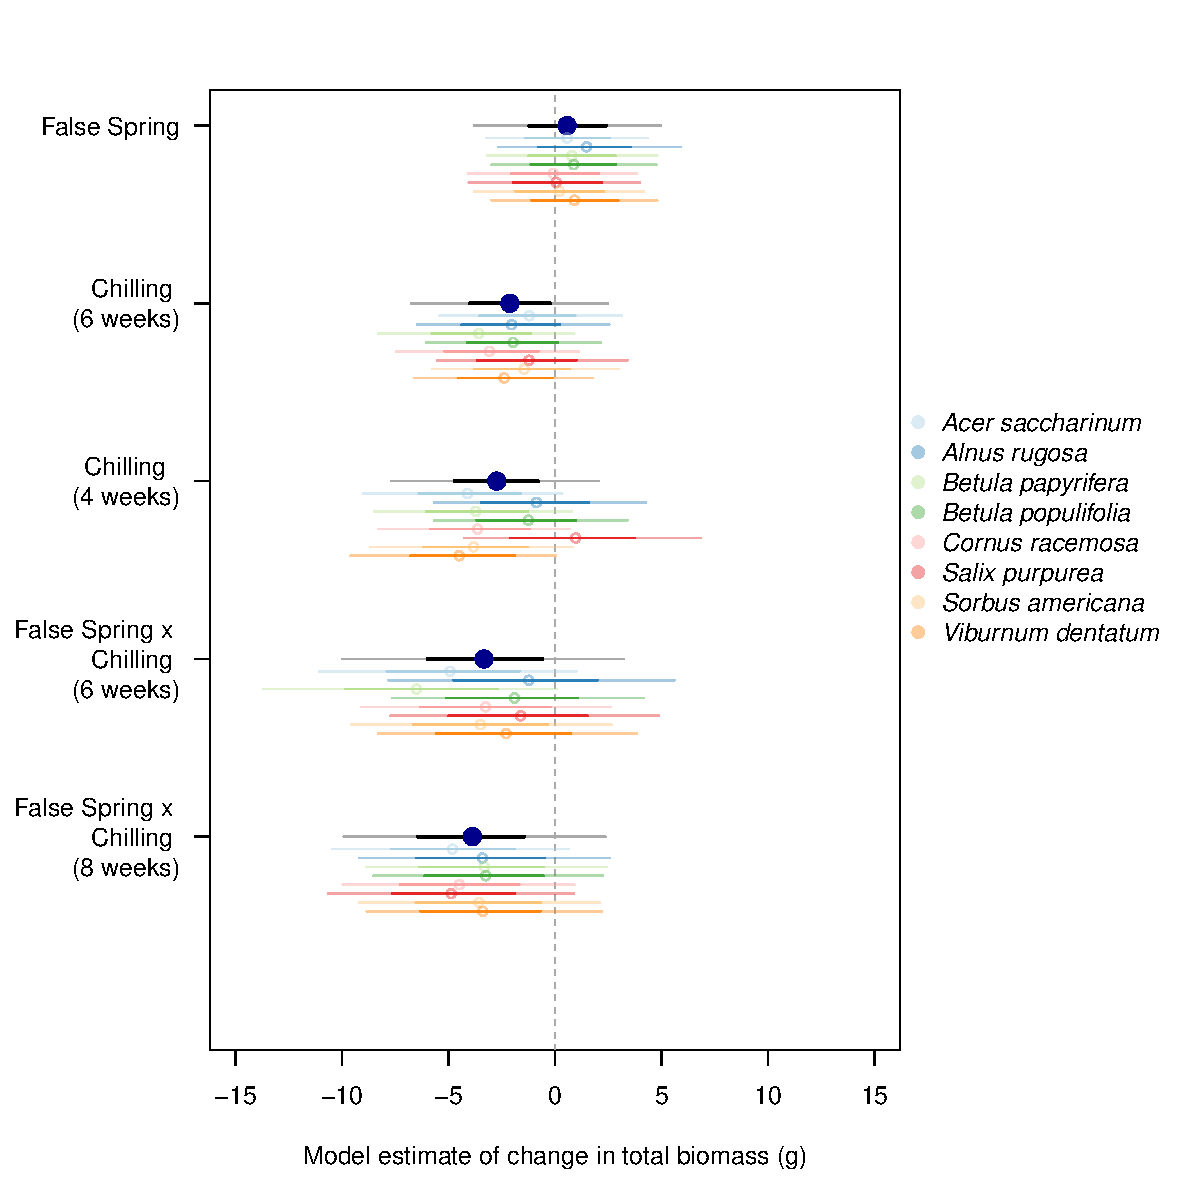
\includegraphics[width=14cm]{..//analyses/figures/totbiomass50and90_brms.pdf} 
  -\caption{Effects of false spring treatment, six weeks of chilling and eight weeks of chilling on total aboveground and belowground biomass (g). }\label{fig:mutotbio}
  -\end{center}
  -\end{figure}}
  
  \newpage
% latex table generated in R 3.6.0 by xtable 1.8-4 package
% Tue Aug 18 10:33:35 2020
\begin{longtable}{lrrrrrrr}
\caption{Summary of model with the effects of false spring treatment and chilling duration across species on leaf chlorophyll content.} \\ 
  \hline
 & mean & 2\% & 10\% & 25\% & 75\% & 90\% & 98\% \\ 
  \hline \endhead  \hline
Intercept & 30.96 & 24.38 & 26.36 & 29.21 & 32.74 & 35.50 & 37.89 \\ 
  Tx & -0.35 & -2.16 & -1.61 & -0.88 & 0.15 & 0.92 & 1.48 \\ 
  Chill 6 Wks & -0.06 & -2.07 & -1.42 & -0.62 & 0.49 & 1.30 & 1.92 \\ 
  Chill 8 Wks & 0.43 & -1.97 & -1.03 & -0.12 & 1.04 & 1.86 & 2.58 \\ 
  Tx:Chill 6 Wks & -1.04 & -3.76 & -2.90 & -1.81 & -0.26 & 0.84 & 1.68 \\ 
  Tx:Chill 8 Wks & -2.11 & -4.74 & -3.88 & -2.81 & -1.40 & -0.36 & 0.31 \\ 
  \textit{Acer saccharinum},Intercept & -5.84 & -12.65 & -10.48 & -7.66 & -4.06 & -1.25 & 1.08 \\ 
  \textit{Alnus incana rugosa},Intercept & 5.66 & -1.33 & 0.96 & 3.81 & 7.48 & 10.35 & 12.40 \\ 
  \textit{Betula papyrifera},Intercept & -2.33 & -9.20 & -6.98 & -4.13 & -0.48 & 2.29 & 4.50 \\ 
  \textit{Betula populifolia},Intercept & 0.68 & -6.50 & -3.99 & -1.12 & 2.48 & 5.33 & 7.54 \\ 
  \textit{Cornus racemosa},Intercept & 0.96 & -5.84 & -3.68 & -0.88 & 2.81 & 5.61 & 7.89 \\ 
  \textit{Salix purpurea},Intercept & 12.24 & 5.25 & 7.55 & 10.37 & 14.05 & 16.89 & 19.14 \\ 
  \textit{Sorbus americana},Intercept & -7.21 & -14.06 & -11.90 & -9.05 & -5.38 & -2.60 & -0.50 \\ 
  \textit{Viburnum dendatum},Intercept & -4.83 & -11.98 & -9.46 & -6.66 & -2.98 & -0.20 & 2.01 \\ 
  \textit{Acer saccharinum},Tx & 0.04 & -1.77 & -0.90 & -0.22 & 0.30 & 1.03 & 1.81 \\ 
  \textit{Alnus incana rugosa},Tx & -0.02 & -1.91 & -1.10 & -0.30 & 0.26 & 1.13 & 1.91 \\ 
  \textit{Betula papyrifera},Tx & -0.19 & -2.44 & -1.40 & -0.44 & 0.13 & 0.69 & 1.34 \\ 
  \textit{Betula populifolia},Tx & -0.10 & -1.99 & -1.22 & -0.36 & 0.18 & 0.88 & 1.54 \\ 
  \textit{Cornus racemosa},Tx & 0.07 & -1.68 & -0.91 & -0.21 & 0.34 & 1.18 & 2.03 \\ 
  \textit{Salix purpurea},Tx & -0.45 & -3.06 & -2.09 & -0.85 & 0.03 & 0.58 & 1.28 \\ 
  \textit{Sorbus americana},Tx & 0.31 & -1.33 & -0.65 & -0.07 & 0.63 & 1.70 & 2.48 \\ 
  \textit{Viburnum dendatum},Tx & 0.30 & -1.22 & -0.58 & -0.06 & 0.59 & 1.62 & 2.55 \\ 
  \textit{Acer saccharinum},Chill 6 Wks & 0.35 & -1.81 & -0.97 & -0.11 & 0.80 & 1.98 & 3.05 \\ 
  \textit{Alnus incana rugosa},Chill 6 Wks & -0.60 & -3.81 & -2.54 & -1.09 & 0.02 & 0.68 & 1.35 \\ 
  \textit{Betula papyrifera},Chill 6 Wks & 0.61 & -1.21 & -0.56 & -0.01 & 1.09 & 2.48 & 3.62 \\ 
  \textit{Betula populifolia},Chill 6 Wks & 0.31 & -1.76 & -0.97 & -0.17 & 0.70 & 2.02 & 3.23 \\ 
  \textit{Cornus racemosa},Chill 6 Wks & -0.38 & -3.37 & -2.16 & -0.81 & 0.12 & 0.95 & 1.75 \\ 
  \textit{Salix purpurea},Chill 6 Wks & -0.73 & -3.84 & -2.76 & -1.33 & -0.01 & 0.67 & 1.52 \\ 
  \textit{Sorbus americana},Chill 6 Wks & 0.11 & -2.52 & -1.41 & -0.33 & 0.58 & 1.65 & 2.77 \\ 
  \textit{Viburnum dendatum},Chill 6 Wks & 0.33 & -1.91 & -0.98 & -0.14 & 0.79 & 1.94 & 2.95 \\ 
  \textit{Acer saccharinum},Chill 8 Wks & 0.04 & -2.46 & -1.51 & -0.43 & 0.47 & 1.61 & 2.85 \\ 
  \textit{Alnus incana rugosa},Chill 8 Wks & 0.33 & -2.20 & -1.18 & -0.21 & 0.85 & 2.15 & 3.31 \\ 
  \textit{Betula papyrifera},Chill 8 Wks & 0.18 & -2.29 & -1.36 & -0.31 & 0.65 & 1.86 & 3.04 \\ 
  \textit{Betula populifolia},Chill 8 Wks & 0.10 & -2.41 & -1.42 & -0.38 & 0.56 & 1.74 & 2.94 \\ 
  \textit{Cornus racemosa},Chill 8 Wks & 1.12 & -0.75 & -0.27 & 0.15 & 1.82 & 3.46 & 4.88 \\ 
  \textit{Salix purpurea},Chill 8 Wks & -0.31 & -3.49 & -2.24 & -0.88 & 0.29 & 1.35 & 2.23 \\ 
  \textit{Sorbus americana},Chill 8 Wks & -0.67 & -3.89 & -2.68 & -1.24 & 0.01 & 0.73 & 1.60 \\ 
  \textit{Viburnum dendatum},Chill 8 Wks & -0.71 & -3.86 & -2.78 & -1.29 & 0.00 & 0.60 & 1.34 \\ 
  \textit{Acer saccharinum},Tx:Chill 6 Wks & 0.15 & -2.87 & -1.64 & -0.38 & 0.70 & 2.05 & 3.36 \\ 
  \textit{Alnus incana rugosa},Tx:Chill 6 Wks & 0.20 & -2.75 & -1.60 & -0.42 & 0.72 & 2.38 & 3.96 \\ 
  \textit{Betula papyrifera},Tx:Chill 6 Wks & 0.08 & -3.05 & -1.80 & -0.44 & 0.61 & 1.97 & 3.09 \\ 
  \textit{Betula populifolia},Tx:Chill 6 Wks & -0.78 & -4.76 & -3.31 & -1.38 & 0.02 & 0.77 & 1.55 \\ 
  \textit{Cornus racemosa},Tx:Chill 6 Wks & 0.27 & -2.46 & -1.46 & -0.29 & 0.78 & 2.32 & 3.82 \\ 
  \textit{Salix purpurea},Tx:Chill 6 Wks & -1.15 & -5.53 & -3.86 & -2.00 & -0.07 & 0.73 & 1.76 \\ 
  \textit{Sorbus americana},Tx:Chill 6 Wks & 0.96 & -1.46 & -0.68 & 0.02 & 1.65 & 3.49 & 5.08 \\ 
  \textit{Viburnum dendatum},Tx:Chill 6 Wks & 0.37 & -2.58 & -1.32 & -0.20 & 0.93 & 2.40 & 3.58 \\ 
  \textit{Acer saccharinum},Tx:Chill 8 Wks & 0.06 & -2.13 & -1.13 & -0.25 & 0.35 & 1.38 & 2.47 \\ 
  \textit{Alnus incana rugosa},Tx:Chill 8 Wks & 0.06 & -2.25 & -1.22 & -0.29 & 0.36 & 1.48 & 2.59 \\ 
  \textit{Betula papyrifera},Tx:Chill 8 Wks & 0.04 & -2.22 & -1.20 & -0.26 & 0.32 & 1.31 & 2.41 \\ 
  \textit{Betula populifolia},Tx:Chill 8 Wks & -0.06 & -2.28 & -1.37 & -0.35 & 0.23 & 1.11 & 1.82 \\ 
  \textit{Cornus racemosa},Tx:Chill 8 Wks & -0.01 & -2.46 & -1.27 & -0.32 & 0.29 & 1.30 & 2.40 \\ 
  \textit{Salix purpurea},Tx:Chill 8 Wks & -0.24 & -3.31 & -2.01 & -0.62 & 0.20 & 1.13 & 2.13 \\ 
  \textit{Sorbus americana},Tx:Chill 8 Wks & 0.05 & -2.33 & -1.30 & -0.27 & 0.39 & 1.44 & 2.54 \\ 
  \textit{Viburnum dendatum},Tx:Chill 8 Wks & 0.11 & -2.08 & -1.12 & -0.22 & 0.42 & 1.51 & 2.74 \\ 
   \hline
\hline
\label{tab:suppmodchl}
\end{longtable}


{\begin{figure} [H]
  -\begin{center}
  -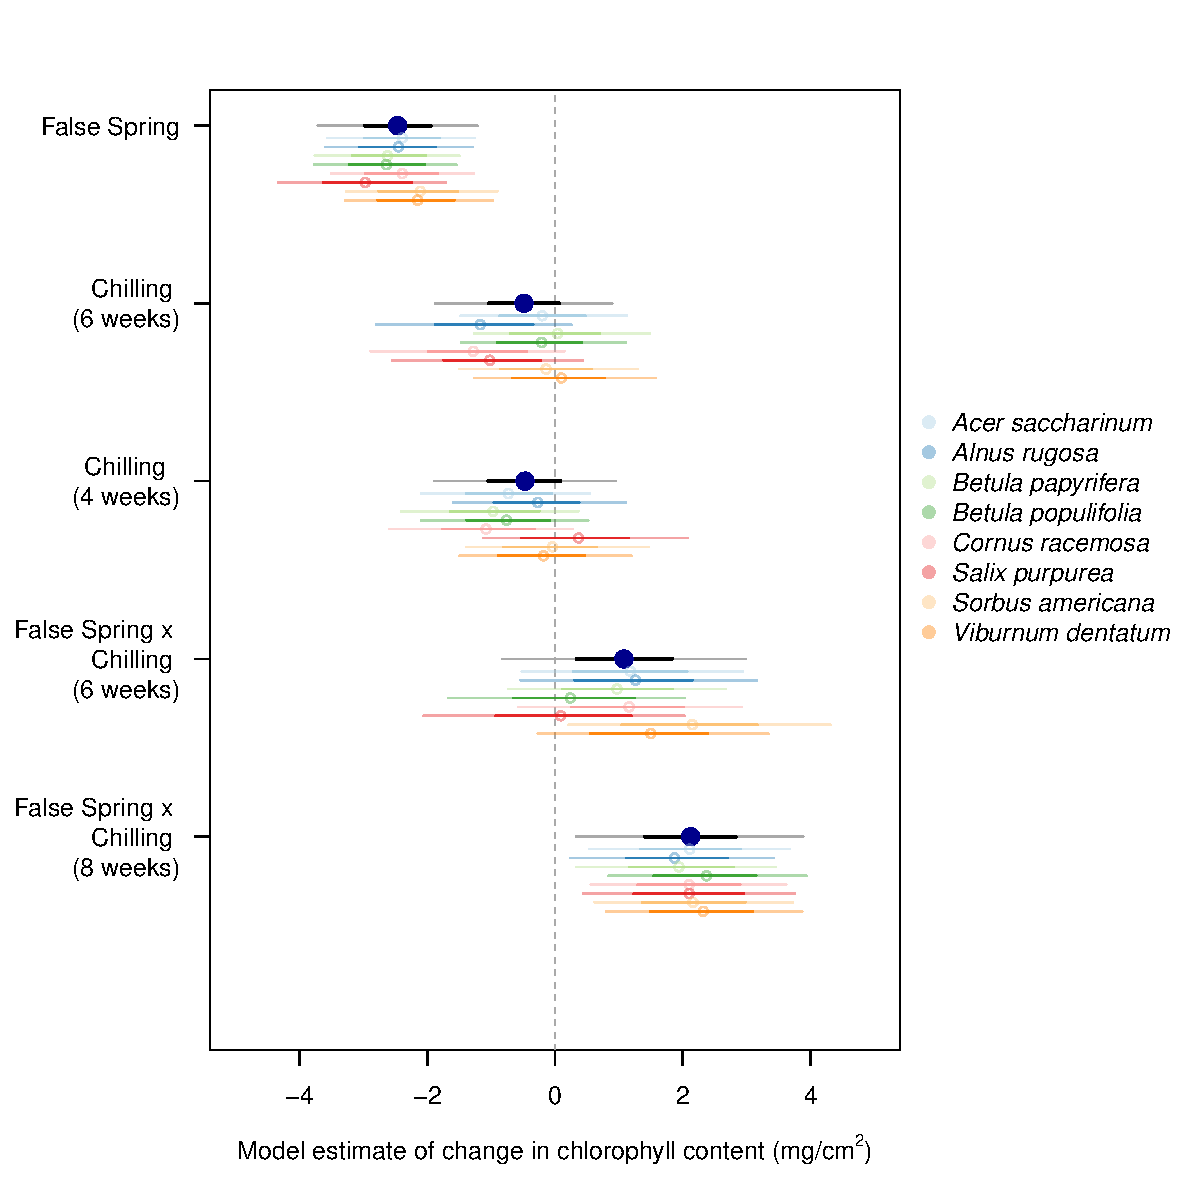
\includegraphics[width=14cm]{..//analyses/figures/chl50and90_brms.pdf} 
  -\caption{Effects of false spring treatment, six weeks of chilling and eight weeks of chilling on chlorophyll content. }\label{fig:muchl}
  -\end{center}
  -\end{figure}}

\newpage
% latex table generated in R 3.6.0 by xtable 1.8-4 package
% Tue Aug 18 10:33:35 2020
\begin{longtable}{lrrrrrrr}
\caption{Summary of model with the effects of false spring treatment and chilling duration across species on leaf toughness.} \\ 
  \hline
 & mean & 2\% & 10\% & 25\% & 75\% & 90\% & 98\% \\ 
  \hline \endhead  \hline
Intercept & 0.43 & 0.27 & 0.33 & 0.39 & 0.47 & 0.53 & 0.59 \\ 
  Tx & -0.05 & -0.10 & -0.08 & -0.06 & -0.04 & -0.02 & -0.00 \\ 
  Chill 6 Wks & -0.06 & -0.11 & -0.09 & -0.07 & -0.05 & -0.03 & -0.02 \\ 
  Chill 8 Wks & -0.05 & -0.11 & -0.09 & -0.07 & -0.04 & -0.02 & -0.00 \\ 
  Tx:Chill 6 Wks & 0.02 & -0.04 & -0.02 & 0.01 & 0.04 & 0.06 & 0.08 \\ 
  Tx:Chill 8 Wks & 0.02 & -0.04 & -0.02 & 0.01 & 0.04 & 0.06 & 0.08 \\ 
  Intercept & 0.37 & 0.22 & 0.27 & 0.34 & 0.41 & 0.47 & 0.53 \\ 
  \textit{Acer saccharinum},Intercept & -0.06 & -0.22 & -0.16 & -0.10 & -0.02 & 0.04 & 0.10 \\ 
  \textit{Alnus incana rugosa},Intercept & -0.05 & -0.21 & -0.15 & -0.09 & -0.01 & 0.05 & 0.11 \\ 
  \textit{Betula papyrifera},Intercept & -0.11 & -0.28 & -0.22 & -0.15 & -0.07 & -0.01 & 0.05 \\ 
  \textit{Betula populifolia},Intercept & -0.10 & -0.27 & -0.20 & -0.14 & -0.06 & 0.01 & 0.06 \\ 
  \textit{Cornus racemosa},Intercept & -0.05 & -0.21 & -0.15 & -0.09 & -0.01 & 0.05 & 0.11 \\ 
  \textit{Salix purpurea},Intercept & 0.15 & -0.01 & 0.05 & 0.11 & 0.19 & 0.26 & 0.32 \\ 
  \textit{Sorbus americana},Intercept & -0.01 & -0.17 & -0.12 & -0.05 & 0.03 & 0.10 & 0.16 \\ 
  \textit{Viburnum dendatum},Intercept & 0.25 & 0.08 & 0.14 & 0.21 & 0.29 & 0.35 & 0.41 \\ 
  \textit{Acer saccharinum},Tx & -0.00 & -0.06 & -0.04 & -0.01 & 0.01 & 0.03 & 0.05 \\ 
  \textit{Alnus incana rugosa},Tx & 0.01 & -0.03 & -0.02 & -0.00 & 0.02 & 0.05 & 0.08 \\ 
  \textit{Betula papyrifera},Tx & 0.01 & -0.05 & -0.03 & -0.00 & 0.02 & 0.04 & 0.06 \\ 
  \textit{Betula populifolia},Tx & 0.01 & -0.05 & -0.03 & -0.01 & 0.02 & 0.04 & 0.06 \\ 
  \textit{Cornus racemosa},Tx & 0.02 & -0.02 & -0.01 & 0.00 & 0.04 & 0.07 & 0.09 \\ 
  \textit{Salix purpurea},Tx & -0.01 & -0.08 & -0.06 & -0.03 & -0.00 & 0.02 & 0.03 \\ 
  \textit{Sorbus americana},Tx & -0.01 & -0.08 & -0.05 & -0.02 & 0.00 & 0.02 & 0.04 \\ 
  \textit{Viburnum dendatum},Tx & -0.02 & -0.09 & -0.07 & -0.03 & -0.00 & 0.01 & 0.03 \\ 
  \textit{Acer saccharinum},Chill 6 Wks & 0.01 & -0.03 & -0.01 & -0.00 & 0.02 & 0.05 & 0.08 \\ 
  \textit{Alnus incana rugosa},Chill 6 Wks & -0.01 & -0.06 & -0.04 & -0.01 & 0.00 & 0.02 & 0.04 \\ 
  \textit{Betula papyrifera},Chill 6 Wks & -0.00 & -0.05 & -0.03 & -0.01 & 0.01 & 0.03 & 0.05 \\ 
  \textit{Betula populifolia},Chill 6 Wks & -0.00 & -0.05 & -0.03 & -0.01 & 0.01 & 0.03 & 0.05 \\ 
  \textit{Cornus racemosa},Chill 6 Wks & -0.01 & -0.07 & -0.04 & -0.02 & 0.00 & 0.02 & 0.04 \\ 
  \textit{Salix purpurea},Chill 6 Wks & 0.01 & -0.04 & -0.02 & -0.00 & 0.01 & 0.04 & 0.07 \\ 
  \textit{Sorbus americana},Chill 6 Wks & -0.01 & -0.07 & -0.05 & -0.02 & 0.00 & 0.02 & 0.03 \\ 
  \textit{Viburnum dendatum},Chill 6 Wks & 0.01 & -0.04 & -0.02 & -0.00 & 0.02 & 0.05 & 0.07 \\ 
  \textit{Acer saccharinum},Chill 8 Wks & 0.02 & -0.03 & -0.01 & 0.00 & 0.04 & 0.07 & 0.10 \\ 
  \textit{Alnus incana rugosa},Chill 8 Wks & -0.02 & -0.09 & -0.06 & -0.03 & 0.00 & 0.02 & 0.04 \\ 
  \textit{Betula papyrifera},Chill 8 Wks & -0.02 & -0.09 & -0.06 & -0.03 & -0.00 & 0.02 & 0.04 \\ 
  \textit{Betula populifolia},Chill 8 Wks & -0.01 & -0.08 & -0.06 & -0.03 & 0.00 & 0.02 & 0.05 \\ 
  \textit{Cornus racemosa},Chill 8 Wks & -0.00 & -0.07 & -0.04 & -0.02 & 0.01 & 0.04 & 0.06 \\ 
  \textit{Salix purpurea},Chill 8 Wks & 0.02 & -0.04 & -0.02 & 0.00 & 0.04 & 0.07 & 0.10 \\ 
  \textit{Sorbus americana},Chill 8 Wks & -0.02 & -0.10 & -0.08 & -0.04 & -0.00 & 0.01 & 0.03 \\ 
  \textit{Viburnum dendatum},Chill 8 Wks & 0.03 & -0.03 & -0.01 & 0.01 & 0.05 & 0.08 & 0.11 \\ 
  \textit{Acer saccharinum},Tx:Chill 6 Wks & 0.01 & -0.05 & -0.03 & -0.00 & 0.01 & 0.05 & 0.08 \\ 
  \textit{Alnus incana rugosa},Tx:Chill 6 Wks & -0.01 & -0.08 & -0.04 & -0.01 & 0.00 & 0.02 & 0.05 \\ 
  \textit{Betula papyrifera},Tx:Chill 6 Wks & -0.00 & -0.08 & -0.04 & -0.01 & 0.01 & 0.03 & 0.05 \\ 
  \textit{Betula populifolia},Tx:Chill 6 Wks & 0.01 & -0.04 & -0.02 & -0.00 & 0.02 & 0.05 & 0.08 \\ 
  \textit{Cornus racemosa},Tx:Chill 6 Wks & 0.00 & -0.05 & -0.03 & -0.01 & 0.01 & 0.04 & 0.08 \\ 
  \textit{Salix purpurea},Tx:Chill 6 Wks & 0.00 & -0.06 & -0.03 & -0.01 & 0.01 & 0.04 & 0.07 \\ 
  \textit{Sorbus americana},Tx:Chill 6 Wks & -0.01 & -0.10 & -0.06 & -0.02 & 0.00 & 0.02 & 0.03 \\ 
  \textit{Viburnum dendatum},Tx:Chill 6 Wks & 0.00 & -0.06 & -0.04 & -0.01 & 0.01 & 0.04 & 0.07 \\ 
  \textit{Acer saccharinum},Tx:Chill 8 Wks & 0.01 & -0.04 & -0.02 & -0.00 & 0.02 & 0.05 & 0.09 \\ 
  \textit{Alnus incana rugosa},Tx:Chill 8 Wks & -0.00 & -0.06 & -0.04 & -0.01 & 0.01 & 0.03 & 0.06 \\ 
  \textit{Betula papyrifera},Tx:Chill 8 Wks & -0.00 & -0.07 & -0.04 & -0.01 & 0.00 & 0.03 & 0.05 \\ 
  \textit{Betula populifolia},Tx:Chill 8 Wks & -0.00 & -0.07 & -0.04 & -0.01 & 0.01 & 0.03 & 0.05 \\ 
  \textit{Cornus racemosa},Tx:Chill 8 Wks & 0.00 & -0.06 & -0.03 & -0.01 & 0.01 & 0.04 & 0.06 \\ 
  \textit{Salix purpurea},Tx:Chill 8 Wks & -0.00 & -0.07 & -0.04 & -0.01 & 0.01 & 0.03 & 0.06 \\ 
  \textit{Sorbus americana},Tx:Chill 8 Wks & -0.00 & -0.06 & -0.04 & -0.01 & 0.01 & 0.03 & 0.06 \\ 
   \hline
\hline
\label{tab:suppmodtough}
\end{longtable}



\newpage
% latex table generated in R 3.6.0 by xtable 1.8-4 package
% Tue Aug 18 10:33:35 2020
\begin{longtable}{lrrrrrrr}
\caption{Summary of model with the effects of false spring treatment and chilling duration across species on leaf thickness.} \\ 
  \hline
 & mean & 2\% & 10\% & 25\% & 75\% & 90\% & 98\% \\ 
  \hline \endhead  \hline
Intercept & 141.76 & 119.08 & 125.87 & 135.57 & 147.79 & 158.06 & 166.29 \\ 
  Tx & -8.90 & -17.68 & -15.08 & -11.29 & -6.46 & -2.75 & 0.29 \\ 
  Chill 6 Wks & 7.21 & -9.50 & -3.49 & 3.16 & 11.24 & 17.94 & 23.06 \\ 
  Chill 8 Wks & -8.38 & -27.21 & -20.39 & -12.84 & -3.67 & 3.68 & 9.06 \\ 
  Tx:Chill 6 Wks & -1.81 & -14.56 & -10.56 & -5.25 & 1.68 & 6.78 & 10.78 \\ 
  Tx:Chill 8 Wks & 1.50 & -10.93 & -7.19 & -2.04 & 5.03 & 9.99 & 13.30 \\ 
  Intercept & 136.92 & 115.60 & 122.45 & 131.52 & 142.58 & 151.41 & 159.60 \\ 
  \textit{Acer saccharinum},Intercept & -31.97 & -57.43 & -49.47 & -38.60 & -25.14 & -15.13 & -7.93 \\ 
  \textit{Alnus incana rugosa},Intercept & 17.84 & -7.75 & 0.82 & 11.24 & 24.62 & 34.74 & 42.97 \\ 
  \textit{Betula papyrifera},Intercept & 32.87 & 6.91 & 15.56 & 26.19 & 39.61 & 49.87 & 58.26 \\ 
  \textit{Betula populifolia},Intercept & 10.53 & -15.48 & -6.66 & 3.71 & 17.31 & 27.75 & 35.83 \\ 
  \textit{Cornus racemosa},Intercept & -8.65 & -33.93 & -25.99 & -15.17 & -1.72 & 8.17 & 15.86 \\ 
  \textit{Salix purpurea},Intercept & 16.74 & -9.31 & -0.19 & 10.08 & 23.41 & 34.04 & 41.29 \\ 
  \textit{Sorbus americana},Intercept & -29.77 & -56.70 & -47.34 & -36.39 & -23.02 & -12.81 & -5.32 \\ 
  \textit{Viburnum dendatum},Intercept & -5.16 & -30.61 & -22.12 & -11.83 & 1.62 & 11.95 & 19.40 \\ 
  \textit{Acer saccharinum},Tx & 0.88 & -7.11 & -4.07 & -0.74 & 2.30 & 7.03 & 11.52 \\ 
  \textit{Alnus incana rugosa},Tx & -2.29 & -15.60 & -10.07 & -3.77 & 0.06 & 1.94 & 3.94 \\ 
  \textit{Betula papyrifera},Tx & 0.77 & -7.33 & -3.99 & -0.85 & 2.11 & 6.87 & 11.80 \\ 
  \textit{Betula populifolia},Tx & -0.08 & -9.56 & -5.28 & -1.47 & 1.27 & 5.04 & 9.39 \\ 
  \textit{Cornus racemosa},Tx & -0.24 & -9.94 & -5.76 & -1.52 & 1.19 & 4.76 & 8.35 \\ 
  \textit{Salix purpurea},Tx & -0.59 & -10.53 & -6.32 & -1.88 & 0.86 & 4.35 & 7.42 \\ 
  \textit{Sorbus americana},Tx & 1.02 & -7.19 & -4.10 & -0.69 & 2.53 & 7.48 & 11.78 \\ 
  \textit{Viburnum dendatum},Tx & 0.12 & -8.94 & -4.91 & -1.21 & 1.40 & 5.24 & 8.93 \\ 
  \textit{Acer saccharinum},Chill 6 Wks & -8.97 & -31.35 & -23.41 & -14.20 & -3.20 & 3.73 & 9.01 \\ 
  \textit{Alnus incana rugosa},Chill 6 Wks & -3.16 & -23.21 & -16.74 & -8.17 & 1.84 & 9.89 & 16.49 \\ 
  \textit{Betula papyrifera},Chill 6 Wks & 1.27 & -18.39 & -11.65 & -3.65 & 6.26 & 14.48 & 21.76 \\ 
  \textit{Betula populifolia},Chill 6 Wks & -1.18 & -21.11 & -14.59 & -6.33 & 3.91 & 11.89 & 18.35 \\ 
  \textit{Cornus racemosa},Chill 6 Wks & 16.15 & -2.21 & 2.08 & 9.80 & 21.75 & 31.67 & 39.11 \\ 
  \textit{Salix purpurea},Chill 6 Wks & -12.29 & -34.05 & -26.76 & -17.63 & -6.61 & 0.61 & 6.97 \\ 
  \textit{Sorbus americana},Chill 6 Wks & 10.65 & -8.06 & -2.47 & 4.73 & 16.11 & 25.45 & 32.65 \\ 
  \textit{Viburnum dendatum},Chill 6 Wks & -1.53 & -21.85 & -15.15 & -6.64 & 3.57 & 11.59 & 17.73 \\ 
  \textit{Acer saccharinum},Chill 8 Wks & 4.24 & -16.95 & -10.58 & -1.50 & 10.03 & 19.20 & 26.80 \\ 
  \textit{Alnus incana rugosa},Chill 8 Wks & -10.03 & -31.69 & -25.10 & -16.00 & -4.07 & 4.54 & 11.62 \\ 
  \textit{Betula papyrifera},Chill 8 Wks & -5.74 & -27.24 & -19.93 & -11.22 & -0.32 & 8.41 & 15.98 \\ 
  \textit{Betula populifolia},Chill 8 Wks & -19.37 & -42.43 & -35.14 & -25.05 & -13.25 & -5.02 & 1.43 \\ 
  \textit{Cornus racemosa},Chill 8 Wks & -3.79 & -26.10 & -18.62 & -9.55 & 1.87 & 10.72 & 18.91 \\ 
  \textit{Salix purpurea},Chill 8 Wks & 0.31 & -21.05 & -14.02 & -5.52 & 5.79 & 15.18 & 23.32 \\ 
  \textit{Sorbus americana},Chill 8 Wks & 19.74 & -1.14 & 4.96 & 13.32 & 25.66 & 35.62 & 44.76 \\ 
  \textit{Viburnum dendatum},Chill 8 Wks & 14.47 & -5.66 & 0.51 & 8.22 & 20.01 & 30.14 & 38.72 \\ 
  \textit{Acer saccharinum},Tx:Chill 6 Wks & 0.81 & -12.64 & -6.83 & -1.36 & 2.79 & 9.69 & 16.74 \\ 
  \textit{Alnus incana rugosa},Tx:Chill 6 Wks & -0.97 & -15.84 & -9.20 & -2.87 & 1.03 & 5.61 & 11.59 \\ 
  \textit{Betula papyrifera},Tx:Chill 6 Wks & 0.45 & -12.44 & -6.54 & -1.66 & 2.29 & 8.77 & 15.03 \\ 
  \textit{Betula populifolia},Tx:Chill 6 Wks & -0.94 & -15.56 & -9.50 & -2.85 & 1.18 & 6.01 & 11.86 \\ 
  \textit{Cornus racemosa},Tx:Chill 6 Wks & -2.00 & -19.11 & -11.82 & -3.90 & 0.53 & 4.34 & 8.85 \\ 
  \textit{Salix purpurea},Tx:Chill 6 Wks & -0.26 & -14.53 & -8.21 & -2.09 & 1.70 & 7.27 & 12.87 \\ 
  \textit{Sorbus americana},Tx:Chill 6 Wks & 0.77 & -12.93 & -7.16 & -1.30 & 2.80 & 9.33 & 16.07 \\ 
  \textit{Viburnum dendatum},Tx:Chill 6 Wks & 1.89 & -8.77 & -4.22 & -0.56 & 3.74 & 11.17 & 18.71 \\ 
  \textit{Acer saccharinum},Tx:Chill 8 Wks & 0.96 & -11.32 & -5.80 & -1.16 & 2.76 & 9.34 & 15.71 \\ 
  \textit{Alnus incana rugosa},Tx:Chill 8 Wks & -0.12 & -12.38 & -7.28 & -1.83 & 1.51 & 6.96 & 13.25 \\ 
  \textit{Betula papyrifera},Tx:Chill 8 Wks & -0.47 & -14.03 & -8.09 & -2.20 & 1.32 & 6.43 & 12.10 \\ 
  \textit{Betula populifolia},Tx:Chill 8 Wks & -0.49 & -14.26 & -8.03 & -2.23 & 1.35 & 6.36 & 11.45 \\ 
  \textit{Cornus racemosa},Tx:Chill 8 Wks & 0.86 & -9.85 & -5.64 & -1.08 & 2.41 & 8.93 & 14.88 \\ 
  \textit{Salix purpurea},Tx:Chill 8 Wks & -1.35 & -15.85 & -10.16 & -3.04 & 0.69 & 4.85 & 9.36 \\ 
  \textit{Sorbus americana},Tx:Chill 8 Wks & 1.31 & -10.34 & -5.38 & -0.88 & 3.13 & 10.00 & 16.75 \\ 
   \hline
\hline
\label{tab:suppmodthick}
\end{longtable}


{\begin{figure} [H]
  -\begin{center}
  -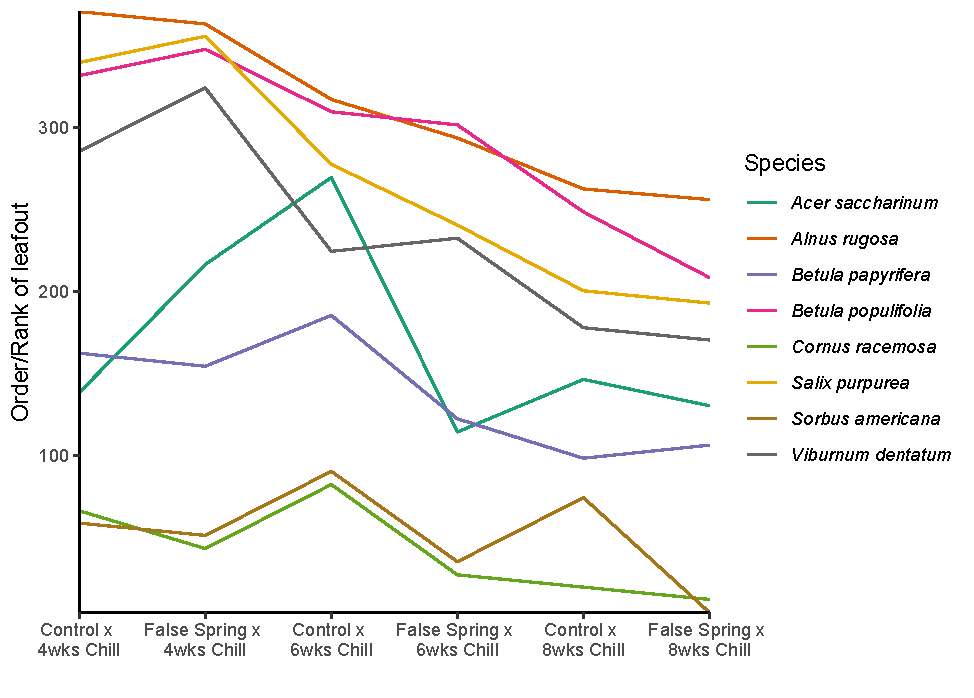
\includegraphics[width=12cm]{..//analyses/figures/budsetorder_byrank.pdf} 
  -\caption{Understanding rank order of leafout across all species using (a) mean trends and (b) raw estimates. }\label{fig:bsetrank}
  -\end{center}
  -\end{figure}}


%%%%% Removed for now
%\newpage






\end{document}
